\documentclass[11pt, a4paper]{article}
\usepackage{pythontex}
\usepackage[german]{babel}
\usepackage{graphicx}
\usepackage{tabularx}
\usepackage{hyperref}
\usepackage{ulem}
\usepackage{subfig}
\usepackage{lastpage}
\usepackage[parfill]{parskip}
\usepackage{framed}
\usepackage{fancyhdr}
% \usepackage{pythontext}
\usepackage[headheight=55pt,
 left=25mm, bottom =25mm]{geometry}

\usepackage{scalerel,stackengine,amsmath}
\newcommand\equalhat{\mathrel{\stackon[1.5pt]{=}{\stretchto{%
    \scalerel*[\widthof{=}]{\wedge}{\rule{1ex}{3ex}}}{0.5ex}}}}


% package to open file containing variables
\usepackage{datatool, filecontents}
\DTLsetseparator{,}% Set the separator between the columns.

% import data
\DTLloaddb[noheader, keys={thekey,thevalue}]{pythonvariables}{pythonvariables.dat}
% Loads mydata.dat with column headers 'thekey' and 'thevalue'
\newcommand{\var}[1]{\DTLfetch{pythonvariables}{thekey}{#1}{thevalue}}

%%%%%% SANS SERIF FONT %%%%%%%%
%\usepackage[OT1]{fontenc}
%\renewcommand*\familydefault{\sfdefault}

%Header Customization
\fancyhead[L]{
\includegraphics[width=0.23\linewidth]{phytax_logo.jpg} \\
}
\fancyhead[C]{\footnotesize
\begin{tabular}{ l }
 Phytax GmbH \\ 
 Wagistrasse 23 \\  
 CH-8952 Schlieren 
\end{tabular}
}

\fancyhead[C]{\footnotesize
 Phytax GmbH \\ 
 Wagistrasse 23 \\  
 CH-8952 Schlieren 
}
\fancyhead[R]{ \footnotesize \noindent \href{mailto:info@phytax.ch}{info@phytax.ch} \\
\href{http://www.phytax.ch}{www.phytax.ch}\\
\href{tel:41434950430}{+41 (0) 43 495 04 30}}

\pagestyle{fancy}
\lfoot[]{\footnotesize Validierungsplan PHYDENT-\DatumRelease}
\rfoot[]{\thepage/\pageref{LastPage} }
\cfoot{}
\renewcommand{\headrulewidth}{0pt}
%%%%%%%%%%%%%%%% VARIABLEN %%%%%%%%%%%%%%%%%%%%%%%%%%%%%
\newcommand\VersionPhEur{10.5}
\newcommand\DatumRelease{20210929}
\newcommand\AnzahlProdukte{227}
\newcommand\VerhaeltnisLernValDaten{73.2:27.8}

\newcommand\NoSpectraRefLearn{5200 (54.2\%)}
\newcommand\NoSpectraRefVal{200 (20.8\%)}
\newcommand\NoSpectraPruef{2400 (25.0\%)}
\newcommand\NrSpektren{7128}
\newcommand\Granulatchargen{396}
\newcommand\NrMatrix{72}
\newcommand\DateRange{2020-2021}


%%%%% Verhaeltnis %%%%%%%

% \newcommand\TotNrLernValData{\NoSpectraRefLearn + \NoSpectraRefVal}

\begin{document}
\section*{Validierungsplan für Prüfungsmethode: PHYDENT-\DatumRelease }

\renewcommand{\arraystretch}{1.2}
\begin{center}
\begin{tabular}{| m{3.5cm} | m{3.5cm}| m{3.5cm} |m{3.5cm}|}
\hline
 & Person & Datum & Visum \\
\hline
Erstellt & & &  \\
& & &\\
\hline
Geprüft & & & \\
& & & \\
\hline
Freigegeben & & & \\
&&&\\
\hline
\end{tabular}
\end{center}




This is document version: \var{document_version}




\subsection*{Zusammenfassung}
PHYDENT ist eine chemometrische Prüfmethode für die Identifikation von Granulaten der Traditionellen Chinesischen Medizin (TCM). PHYDENT ist vorgesehen für die Ausgangstoffprüfung gemäß deutscher Apothekenbetriebsordnung (§§ 6, 7 und 11). Die Prüfmethode ist ausgelegt für die Identifikation von Granulatprodukten verschiedener Hersteller basierend auf spektralen Merkmalen im Mittleren Infrarot (MIR; 400–4000 cm$^{-1}$). Die Methode wurde entwickelt zur Verwendung mit Infrarot-Spektrometern der ALPHA Produktereihe (Bruker, Deutschland). Dieses Dokument beschreibt den Validierungsplan für PHYDENT gemäß ICH (Q2)R1 sowie den Bestimmungen des Europäischen Arzneibuchs (\VersionPhEur). Die Methodenvalidierung umfasst Prüfungen zu Spezifität und weiteren kritischen Parametern.


\subsection*{Zweck}
Dieser Validierungsplan beschreibt die analytische Testmethode PHYDENT-\DatumRelease, im Folgenden PHYDENT genannt, sowie die Strategie und Akzeptanzkriterien für deren Validierung.

\newpage
\tableofcontents

\newpage

\section{Beschreibung der Methode}
PHYDENT ist eine computergestützte chemometrische Methode für die infrarotspektroskopische Identifikation von Granulaten der Traditionellen Chinesischen Medizin\footnote{Bei Granulaten handelt es sich in der Regel um wässrige Rohdrogen-Extrakte, welche auf eine Trägersubstanz (z.B. Maisstärke) aufgezogen sind.}. Die Methode ist ausgelegt für die Identifikation von \AnzahlProdukte\ Granulatprodukten unterschiedlicher Hersteller nach deutscher Apothekenbetriebsordnung\footnote{TCM-Granulate gelten als Ausgangstoffe im Sinne der ApBetrO § 7, da Patienten üblicherweise Rezepturen aus mehreren Granulaten verschrieben werden. Demzufolge ist auch bei Vorliegen eines GMP-konformen Prüfzertifikats für jedes Rezepturgranulat eine nochmalige Identitätsprüfung in der Apotheke erforderlich (ApBetrO §§ 6 \& 11).}.  PHYDENT stellt gemäß Ph.Eur. (\VersionPhEur; 5.21) eine Analyse mit Kontrollfunktion dar, bei welcher die Zugehörigkeit zu bekannten Klassen vorhergesagt wird. Die Eingabedaten der Prüfmethode sind spektrale Probenmerkmale im Mittleren Infrarot (MIR, 400 - 4000 cm$^{-1}$), die Ausgabe ist die Produkteidentität von TCM Granulaten.



\subsection{Geltungsbereich}

\textbf{Proben}: PHYDENT ist ausgelegt für die Identifikation von definierten Chargen von 227 Granulatprodukten unterschiedlicher Hersteller (Anhang \ref{append:Liste_ unterstützte_Produkte}, \ref{append:Liste_unterstützte_Chargen})\footnote{Die Identifikation von unbekannten Chargen ist nicht vorgesehen. Grund hierfür ist, trotz standardisierter Herstellungsbedingungen dass mehrere Chargen desselben Produkts signifikante spektrale Variabilität aufweisen können (z.B. aufgrund von Unterschieden in den dafür verwendeten Rohstoffen).}.  Die Methode muss fähig sein, unbekannte Gebinde dieser Chargen zu identifizieren (Generalisierung auf Ebene des Gebindes). \\

\textbf{Gerät/Analyst}: Die Methode ist vorgesehen für die Verwendung mit der ALPHA/Platinum-ATR-Messplattform (Bruker). Die Methode muss Unabhängig des Geräts und unabhängig des Analysten dieselben Resultate erzielen (Generalisierung auf Ebene des Geräts und des Analysten).

\textbf{Verwendungsszenario} (Abbildung (\ref{fig:Flussdiagram})):
\begin{enumerate}
\item Ein TCM-Granulat wird an eine Apotheke geliefert. Der Lieferung liegt ein GMP-konformes Prüfzertifikat bei. Das Zertifikat bezeugt unter anderem die Arzneibuch-konforme Identifikationprüfung der Charge mittels Hochleistungsdünnschichtchromatographie (2.8.25).
\item Die Wareneingangskontrolle und Probennahme der zu prüfenden Granulate erfolgt nach apothekeninternem Qualitätssicherungssystem.
\item Das versiegelte Gebinde wird geöffnet und eine kleine Probenmenge (Spatelspitze) zur Messung entnommen. Die Messung wird auf der ALPHA/Platinum ATR Messplattform ausgeführt (Bruker, Deutschland).
\item Direkt im Anschluss an die Messung identifiziert die jeweils aktuelle Version von PHYDENT automatisch das Granulatprodukt. Die Analyseergebnisse werden gespeichert und werden dokumentiert.
\end{enumerate}

\begin{figure}
\centering
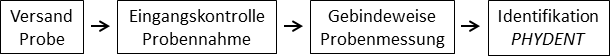
\includegraphics[width=0.8\textwidth]{flussdiagram.png}
\caption{Flussdiagramm Verwendungsszenarion}
\label{fig:Flussdiagram}
\end{figure}

\subsection{Referenzen}
TCM-Granulate gelten gemäß Europäischem Arzneibuch als „Extrakte aus pflanzlichen Drogen“ (\VersionPhEur; 0765). Für Granulate liegen keine Einzelmonographien vor. Deshalb können für Infrarot-basierte Identifikationsmethoden gemäß Europäischem Arzneibuch (\VersionPhEur; 2.2.24) geeignete Referenzstandards definiert und verwendet werden.

\subsubsection{Granulate}
Alle Produktchargen wurden durch Phytax GmbH gemäß den Bestimmungen des jeweils aktuellen Europäischen Arzneibuchs (0765; 2.8.25), sowie nach internen Qualitätsmanagementsystem (SOPs 3.2.3, 3.6.6 und 3.6.7) einwandfrei geprüft. Die Prüfung der Referenzen erfolgte jeweils zusammen mit dem entsprechenden, durch den Granulathersteller zur Verfügung gestellten, Ausgangsmaterial (Rohdroge). Somit ist die Rückverfolgbarkeit auf das jeweilige Ausgangsmaterial gewährleistet.

\subsubsection{Hilfsstoffe}
\label{sec:Hilfsstoffe}
Die für die Granulat-Produktepalette verwendeten Hilfsstoffe sind Cellulose, Cyclodextrin, Laktose und Maisstärke. Diese Hilfsstoffe werden in der Methodenentwicklung und Methodenprüfung berücksichtigt (vgl. Kap. \ref{sec:Sampling_Design}).

\subsection{Spektraldaten}
Die Probenmessung erfolgte gemäß internem Qualitätsmanagementsystem (SOP 3.7.1) sowie den Bestimmungen des jeweils gültigen Europäischen Arzneibuchs (2.2.24). Für die Modellierung von PHYDENT wurden insgesamt \NrSpektren\ Spektren von \Granulatchargen\ Granulatchargen (\AnzahlProdukte\ Produkte) verwendet (Anhänge \ref{append:Liste_ unterstützte_Produkte}, \ref{append:Liste_unterstützte_Chargen}). Nebst diesen Produktspektren wurden insgesamt \NrMatrix\ Spektren von vier in der Granulatherstellung gängig verwendeten Hilfsstoffen einbezogen. Die Spektraldaten wurden ausgewogen auf zwei baugleichen Spektrometern (ALPHA / Platinum ATR; Bruker) durch fünf Analysten \DateRange\ gemessen (Anhang \ref{append:Weitere_kritische_Parameter}).

\subsubsection{Sampling Design}
\label{sec:Sampling_Design}
Der Datensatz zur Entwicklung der Methode (Lern-/Validierungsdaten) besteht aus insgesamt 7200 Spektren (Anhang \ref{append:Spektren_Lern-/Validierungsdaten}), wobei die Lerndaten und Validierungsdaten in einem Verhältnis von 73.2:27.8. aufgeteilt wurden. Zur Überprüfung der Leistungsfähigkeit der Methode sollen ferner unabhängige Prüfdaten mit einem Umfang von mindestens 20\% der L/V-Daten verwendet werden (Tabelle \ref{tab:Aufteilung_gesamtdaten}). Der gesamte Datensatz soll ausgeglichen auf zwei baugleichen Spektrometern gemessen werden (Generalisierung auf Geräteebene). Abbildung \ref{fig:Sampling_Design} zeigt eine Übersicht des angewendeten Sampling Designs.

\begin{table}
\begin{center}
\begin{tabular}{| m{7cm} | m{7cm}| }
\hline
Datensatz & Anzahl Spektren \\
\hline
1) Lerndaten & \NoSpectraRefLearn \\
\hline
2) Validierungsdaten (hold-out) & \NoSpectraRefVal \\
\hline
3) Unabhängige Prüfdaten & \NoSpectraPruef \\
\hline
\end{tabular}
\end{center}
\caption{Aufteilung der Gesamtdaten zur Entwicklung und Überprüfung der Methode}
\label{tab:Aufteilung_gesamtdaten}
\end{table}

\textbf{Produkte}\\[1.2pt]
Gemäß Anwendungsszenario muss PHYDENT fähig sein, unbekannte Gebinde von bekannten bzw. unterstützen Produktechargen zu erkennen (Generalisierung auf Gebindeebene). Deshalb werden den Lern- \& Validierungsdaten (L\&V) und den Prüfdaten (P) für jede Produktecharge unabhängige Gebinde zugewiesen. Für die L\&V-Daten wurde pro Produktecharge ein Gebinde gemessen; für die P-Daten werden zusätzliche ein weiteres unabhängige Gebinde gemessen (pro Gerät je 3-fach wiederholt).

\textbf{Hilfsstoffe}\\[1.2pt]
Granulat-Hilfsstoffe sind potentielle Verfälschungen von Granulatprodukten und werden deshalb in der Methodenentwicklung einbezogen (Negativkontrolle). Total \NrMatrix\ Spektren der in Kap. \ref{sec:Hilfsstoffe} beschriebenen Hilfsstoffe wurden ausgewogen auf zwei baugleichen Spektrometern gemessen (pro Charge je 6-fach wiederholt) und den L\&V- Daten zugewiesen. Unabhängige Messungen derselben Hilfstoffe werden den P-Daten zwecks besserer Identifikation bzw. Zurückweisung zugewiesen.

\textbf{Blank}\\[1.2pt]
Messung des unbedeckten Sensors (Leermessung/Blank) ist ein möglicher Messfehler. Um falsche Identifikationsresultate aufgrund einer unbeabsichtigten Leermessung auszuschliessen, werden Blank-Messungen den P-Daten zugewiesen (Negativkontrolle). Blankmessungen wurden auf zwei baugleichen Spektrometern erstellt (je 6-fach wiederholt).
 
\begin{figure}[h]
\begin{center}
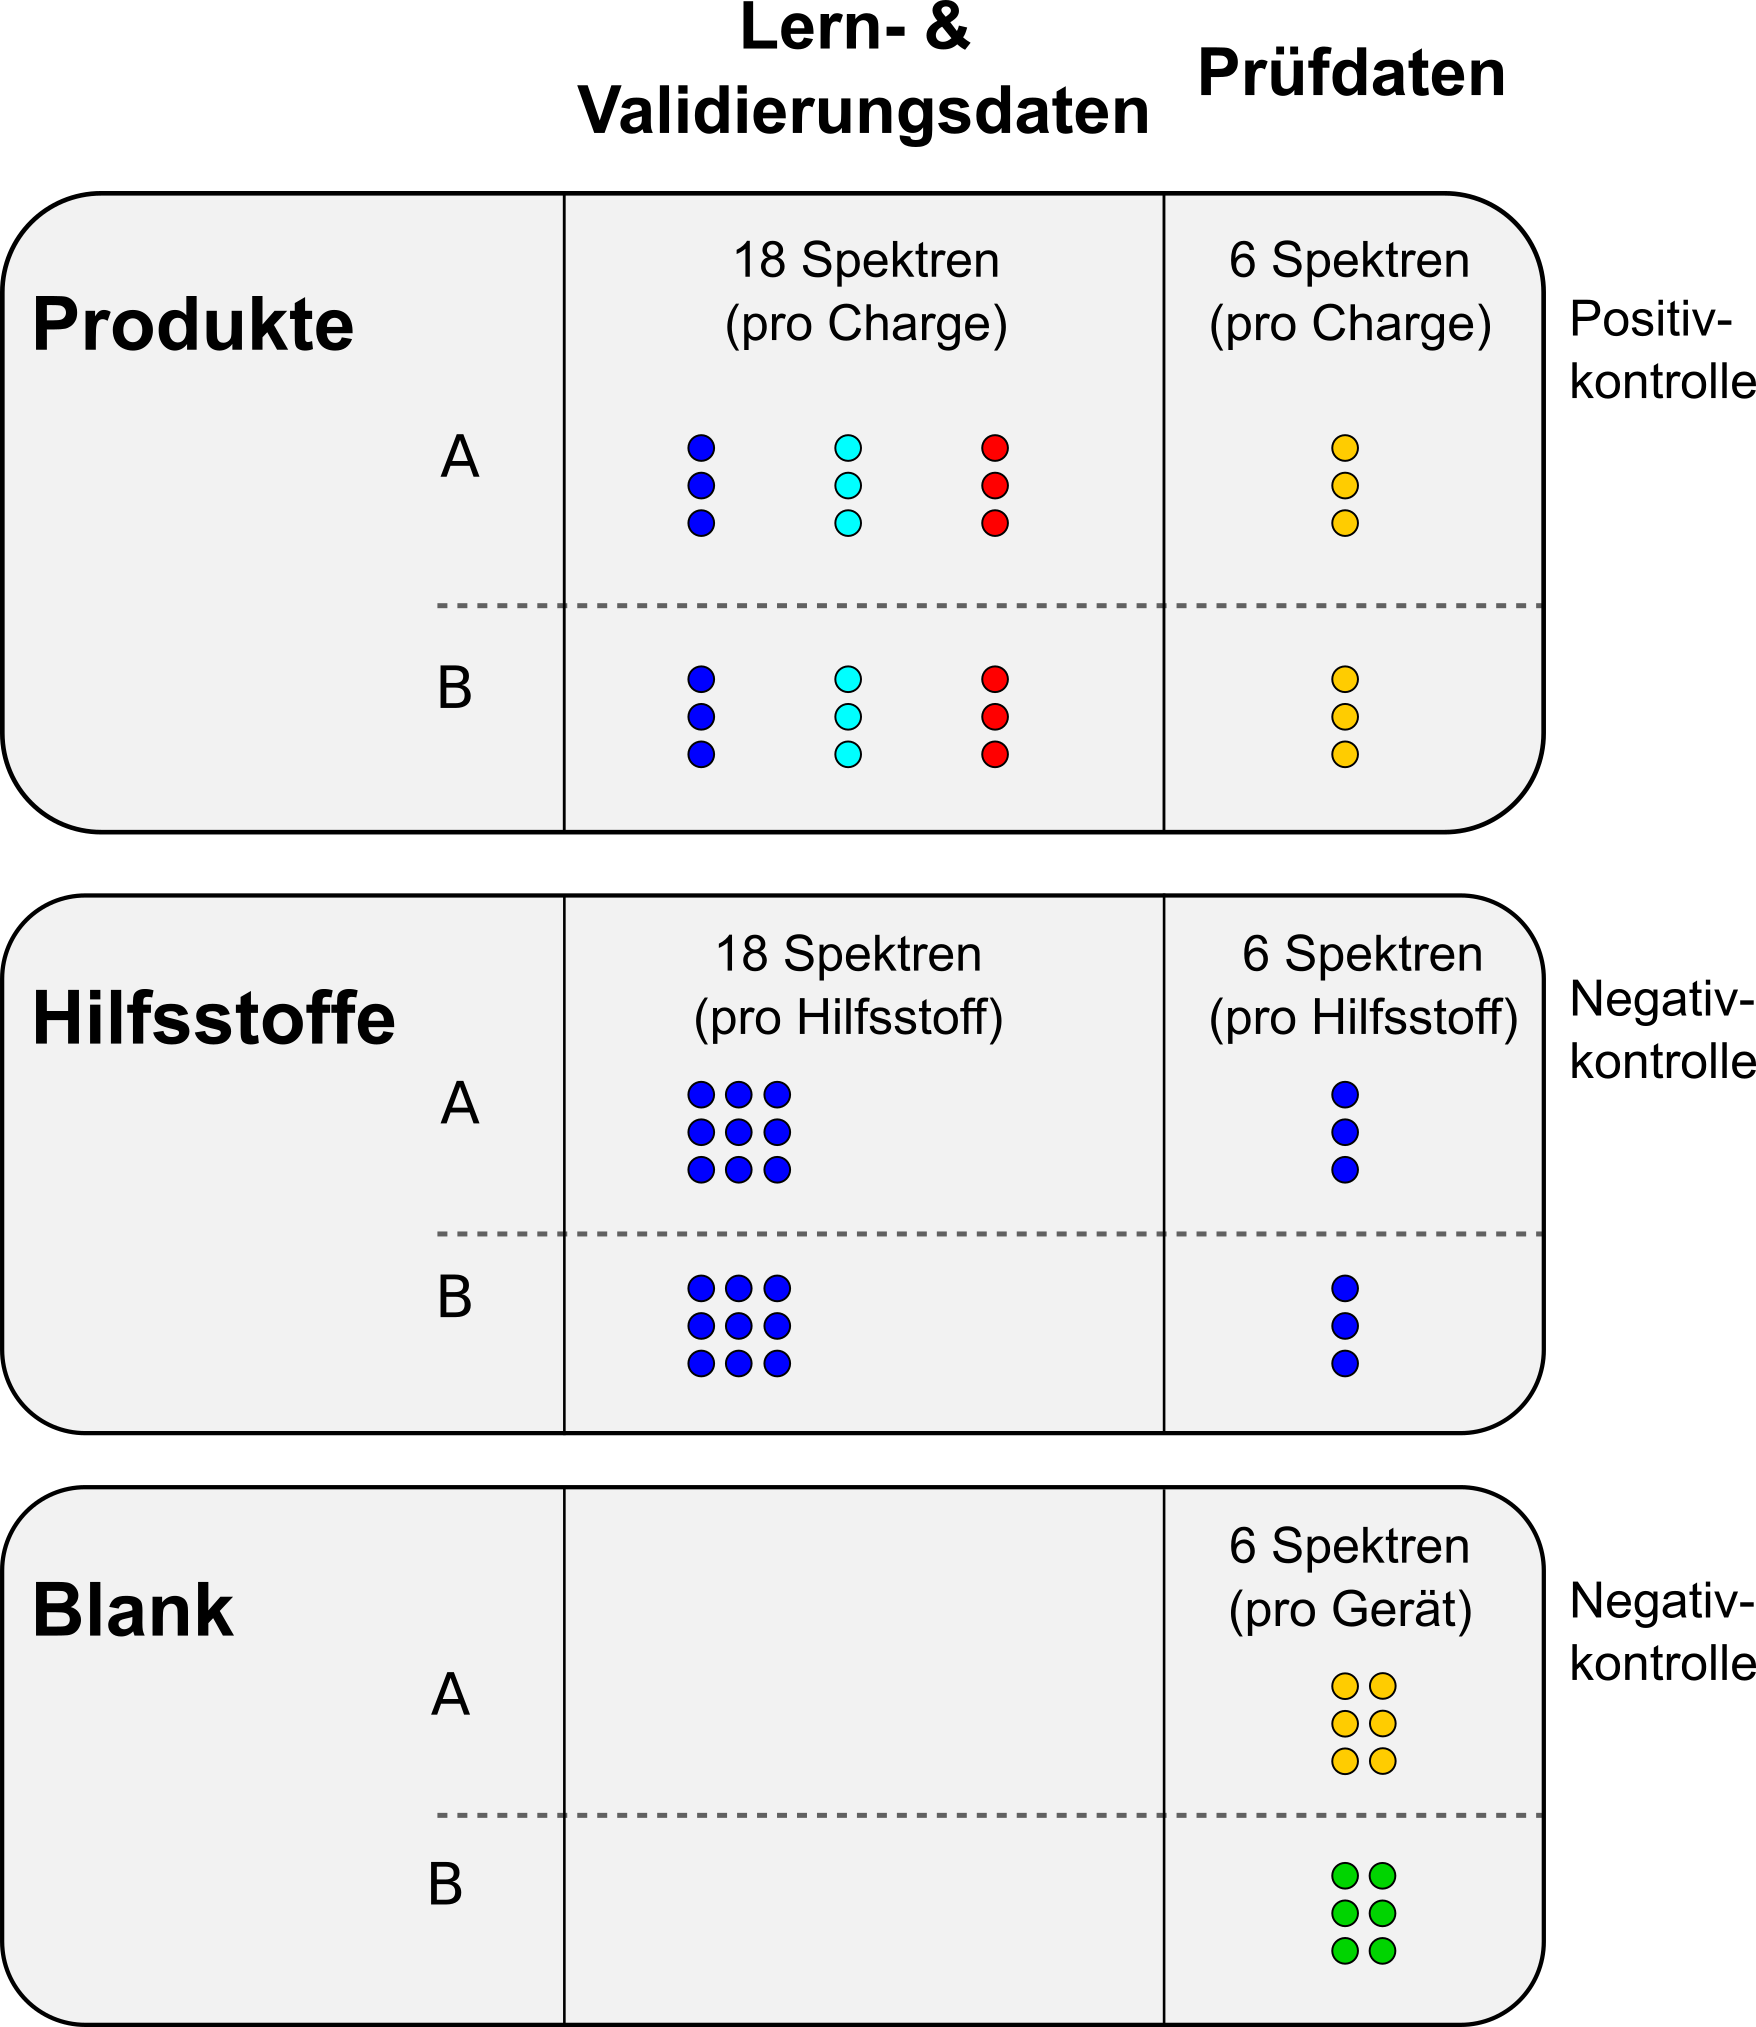
\includegraphics[width=0.8\textwidth]{sampling_design.png}
\end{center}
\caption{Übersicht zum Sampling Design. Alle Spektren werden ausgewogen auf zwei baugleichen Geräten gemessen (A/B). Die Prüfdaten der Granulatprodukte bestehen aus Messungen von Gebinden, welche nicht für die Modellierung (L/V-Daten) verwendet wurden.
Kreis = Einzelne Messung, Farbe = Unterschiedliche Gebinde, A/B = Gerätecode
}
\label{fig:Sampling_Design}
\end{figure}

\subsection{Methodenentwicklung}
PHYDENT besteht aus hierarchisch ineinander geschachtelten Künstlichen Neuronalen Netzen\footnote{Künstliche Neuronale Netze sind ein wichtiges Werkzeug zur Mustererkennung in der quantitativen Datenanalyse. Das grundlegende Element eines KNN, das künstliche Neuron, kann als ein mathematisches Verfahren verstanden werden, das als Eingabe die Summe eines gewichteten Vektors und einer Verzerrung (Bias) verwendet. Für eine detaillierte Einführung in KNN siehe z.B. Priddy und Keller (2009).} (KNN). Die Methodenentwicklung erfolgte nach internem Qualitätsmanagementsystem (SOP 3.7.3) sowie den Bestimmungen des jeweils gültigen Europäischen Arzneibuchs (5.21). Anhang \ref{append:Chemometrische_Verfahren} beschreibt die einzelnen relevanten Bestimmungen des Europäischen Arzneibuchs hinsichtlich der Entwicklung chemometrischer Verfahren (5.21), und erläutert, wie diese für die vorliegende Methode berücksichtigt wurden. Anhang \ref{append:IR-Spektropskopie} beschreibt die einzelnen relevanten Bestimmungen des Europäischen Arzneibuchs zur Verwendung der Infrarot-Spektroskopie (2.2.24), und diskutiert wie diese für PHYDENT berücksichtigt wurden. Die Datenanalyse sowie die Entwicklung der Methode erfolgte unter Zuhilfenahme von NeuroDeveloper (Synthon Analytics, Deutschland) und R (R Core Team 2020).

\subsection{Systemeignungstest}
Die Kontrolle der Leistungsfähigkeit der Spektrometer erfolgt laufend gemäß Europäischem Arzneibuch (\VersionPhEur; 2.2.24). Dazu gehören regelmäßige (wöchentliche bzw. jährliche) Performance Qualification (PQ) und Operational Qualification (OQ) Tests mit geräteinternen Testroutinen. Die Tests umfassen die Prüfpunkte 1) Richtigkeit der Wellenzahlskala (Polystyrol/Wasserdampf); 2) Spektrale Auflösung; 3) 100\%-Linie; 4) Empfindlichkeit; sowie 5) Signal-Rauschen-Verhältnis.


\section{Vorgehen}
\label{sec:Vorgehen}
Die Methodenvalidierung erfolgt gemäß internationalen Richtlinien (ICH Guideline Q2R1) sowie dem aktuellem Europäischem Arzneibuch (\VersionPhEur). Die für die Validierung relevanten Prüfpunkte umfassen Selektivität/Spezifität und weitere kritische Parameter. Robustheit (Probentemperatur und Probenfeuchtigkeit) werden als nicht kritisch erachtet (s. Kapitel \ref{sec:Robustheit}). In Anlehnung an die Bestimmungen des Europäischen Arzneibuchs (5.21) wird der gesamte Datensatz unterteilt in 1) Lerndaten, 2) Validierungsdaten und 3) Unabhängige Prüfdaten

\begin{figure}[h]
\begin{center}
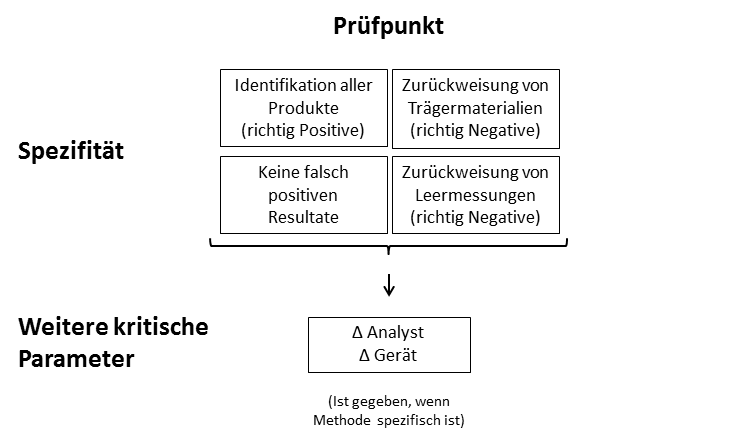
\includegraphics[width=0.8\textwidth]{flussdiagram2.png}
\end{center}
\caption{Flussdiagramm zur Überprüfung der einzelnen Parameter}
\label{fig:Sampling_Design}
\end{figure}

\subsection{Selektivität / Spezifität}
Die Validierung von Identifikationsmethoden verlangt gemäß ICH Richtlinien den Nachweis von Selektivität/Spezifität, wobei eine Methode nur dann selektiv/spezifisch ist, wenn sie die Analyten eindeutig von zu erwartenden anderen Analyten bzw. Verfälschungen unterscheidet (ICH Guideline Q2R1). Für die vorliegende Validierung wurde Selektivität der Methode folgendermaßen definiert:
\begin{enumerate}
\item 	Fähigkeit, alle unterstützten Granulatprodukte korrekt zu identifizieren;
\item 	Fähigkeit, zu erwartende Verfälschungen (Hilfsstoffe und Produkte mit künstlich beigemischtem Hilfststoff) korrekt zurückzuweisen;
\item	Fähigkeit, Leermessungen korrekt zurückzuweisen.
\end{enumerate}

\subsection{Robustheit}
\label{sec:Robustheit}
\textbf{Probentemperatur}\\[1.2pt]
Probentemperatur wird als nicht kritisch erachtet, da aufgrund der geringen Probenmenge sowie der Messtechnik (ATR, abgeschwächte Totalreflexion) davon ausgegangen werden kann, dass sich die Temperatur der Probe während des Messvorgangs jener des Geräts angleicht (Anhang \ref{append:Weitere_kritische_Parameter}).

\textbf{Probenfeuchtigkeit}\\[1.2pt]
Probenfeuchtigkeit wird ebenfalls als nicht kritisch betrachtet, da die Versiegelung von Probengebinden gemäß Verwendungsszenario jeweils unmittelbar vor der Messung entfernt wird. Einfluss von Variation in Probenfeuchtigkeit auf das Mess- und Analyseergebnis kann somit ausgeschlossen werden (Anhang \ref{append:Weitere_kritische_Parameter}).


\subsection{Weitere kritische Parameter}
Folgende Parameter werden als potentiell kritisch eingestuft und sollen bei der Validierung berücksichtigt werden:

\textbf{Vergleichspräzision} \\[1.2pt]
Vergleichspräzision beschreibt die Präzision unter Vergleichsbedingungen. „Vergleichsbedingungen […] sind Bedingungen, unter denen Ermittlungsergebnisse mit demselben Verfahren, an identischem Material (selbe Probe), aber in verschiedenen Labors, von verschiedenen Bearbeitern und mit verschiedener Geräteausrüstung erhalten werden“. (Kromidas 2000, s.49, Hervorh. im Original) \\

Vergleichspräzision wurde berücksichtigt indem der Gesamtdatensatz auf zwei baugleichen Geräten von verschiedenen Analysten gemessen wird. Geräte- sowie Analystenunabhängigkeit wird nicht direkt gezeigt, sondern indirekt als gegeben angenommen, sofern die Methode selektiv ist.


\subsection{Prüfkriterien}
\label{sec:Prüfkriterien}
Für die Beurteilung jedes Spektrums des Prüfdatensatzes werden folgende etablierte Prüfkriterien berücksichtigt (cf. Udelhoven et al. 2003, Fahlmann 1988):

\textbf{WTA}\\[1.2pt]
WTA steht für «Winner takes all» und bedeutet, dass die höchste Aktivierung\footnote{Jedes Neuron verfügt über eine Aktivierungsfunktion, anhand von welcher eine Eingabe in eine Ausgabe umgerechnet wird.}, d.h. die Aktivierung des Siegerneurons\footnote{Der Begriff “Neuron” bezieht sich auf die kleinste funktionale Einheit eines Künstlichen Neuronalen Netzes. Das Siegerneuron ist jenes Neuron der Ausgabe-Schicht, welches über die höchste Aktivierung verfügt.}, die Identifikation bestimmt. Das WTA-Kriterium ist nur dann erfüllt, wenn der Aktivierungswert des Siegerneurons mindestens 0.7 und die Distanz zum Aktivierungswert des zweitbesten Neurons mindestens 0.3 beträgt. Dieses Kriterium stellt sicher, dass die Identifikation hinreichend eindeutig ist.\\

\textbf{40-20-40}\\[1.2pt]
Dieses Kriterium besagt, dass das Siegerneuron eine Aktivierung von mindestens 0.6 aufweisen muss und die Aktivierung der restlichen Neuronen 0.4 nicht übersteigen darf. Dieses Kriterium stellt sicher, dass die Identifikation hinreichend eindeutig ist. \\

\textbf{Extrapolation}\\[1.2pt]
Dieses Kriterium beschreibt die Euklidische Distanz eines Prüfspektrums zum Klassenzentroid im Verhältnis zur maximalen Distanz der Trainingsspektren zum Klassenzentroid. Das Kriterium gilt als erfüllt, wenn der Extrapolationswert eines Spektrums $\leq 200\%$ beträgt. \\

Für jede Identifikation, werden die oben beschriebenen Prüfkriterien nach folgender Heuristik beurteilt (cf. Udelhoven et al. 2003): Eine Identifikation findet statt, falls sowohl das Extrapolation-Kriterium, als auch mindestens entweder das WTA- oder das 40-20-40-Kriterium erfüllt sind. Umgekehrt gilt eine Identifikation als fehlgeschlagen, falls das Extrapolation-Kriterium nicht zutrifft, oder falls sowohl das WTA-, als auch das 40-20-40-Kriterium nicht zutreffen. Jeder Einzeltest wird dokumentiert.

\section{Aktzeptanzkriterien}
Die Validierung gilt als bestanden falls:

\begin{enumerate}
\item Mindestens $99\%$ aller Einzelmessungen des Prüfdatensatzes korrekt identifiziert werden;
\item keine falsch positiven Resultate auftreten;
\item alle Blankmessungen korrekt zurückgewiesen werden (richtig negativ);
\item alle Trägermaterial-Spektren korrekt zurückgewiesen werden (richtig negativ);
\item Produktemischungen mit einem zusätzlichen Trägermasse-Anteil von $> 20\%$  bei mindestens der Hälfte der Messungen (Sechsfachbestimmung) korrekt zurückgewiesen wird.
\end{enumerate}


\subsection{Vorgehen}
\begin{enumerate}
\item Bestimmung/Messung der für die Prüfgruppe verwendeten Daten. Jede Produktcharge soll mit mindestens zwei von den Lern-/Validierungsdaten unabhängigen Gebinden als Positivkontrolle im Prüfdatensatz repräsentiert sein. Ebenfalls sollen Trägermaterialien (Hilfsstoffe) und Leermessungen (negative Referenzen) getestet werden.
\item Testen der Selektivität und Generalisierbarkeit auf Gebindeebene anhand des Prüfdatensatzes. Für jedes Spektrum des Prüfdatensatzes sollen die in Kapitel \ref{sec:Prüfkriterien} beschriebenen Prüfkriterien evaluiert werden.
\item Indirekte Beurteilung von Vergleichspräzision (weitere kritische Parameter) gemeinsam mit Selektivität.
\item Auswertung der Resultate und Gesamtbeurteilung der Methode
\end{enumerate}


\section{Dokumentation, Auswertung und Validierungsbericht}
Die Dokumentation der Methodenvalidierung erfolgt gemäß internem Qualitätssicherungssytem (SOPs 1.11.1, 6.1.1 und 6.3.1).


\section{Besondere Bestimmungen}
Keine.

\section{Verantwortlichkeiten}
\uline{Validierungsverantwortliche Personen:}\\
Dr. Peter Staub (Phytax GmbH, Schlieren)

\uline{Fachtechnisch verantwortliche Person:}\\
Dr. Shu-Yuan Wang-Tschen(Phytax GmbH, Schlieren)

\uline{Externe Beratung:}\\
Dr. Jürgen Schmitt (Synthon Analytics GmbH, Heidelberg)


\section{Geräte und Software}
\begin{itemize}
\item ALPHA Spektrometer Basismodul (Bruker; Gerätenr. G092; Seriennr. 101938)
\item ALPHA Spektrometer Basismodul (Bruker; Gerätenr. G164; Seriennr. 105305)
\item ALPHA Platinum ATR Messmodul (Bruker; Gerätenr. G092; Seriennr. 101938)
\item ALPHA Platinum ATR Messmodul (Bruker; Gerätenr. G164; Seriennr. 105305)
\item OPUS Software Suite (Version 8.5; Bruker)
\item NeuroDeveloper Software (Version 2.6; Synthon Analytics)
\item R
\end{itemize}


\section{Referenzen und mitgeltende Unterlagen}
\begin{itemize}
\item SOP 1.11.1 „Dokumentation“
\item SOP 3.2.3 „Dünnschichtchromatographie”
\item SOP 3.6.6 „Referenzen für DC-Identitätsbestimmungen“
\item SOP 3.6.7 „Produktspezifische DC-Referenzmuster”
\item SOP 3.7.1 „MIR Spektroskopie“
\item SOP 3.7.3 „FTIR-basierte Prüfmethoden der zweiten Identifikationsreihe“
\item SOP 6.1.1 „Validierungsmasterplan“
\item SOP 6.2.8 „Qualifizierung Infrarotspektrometer“
\item SOP 6.3.1 „Methodenvalidierung“
\item SOP 6.8.13 „Zugriffsregelung des IR Spektrometers“
\item Arbeitsanweisung 3.7.1.A1 „MIR Methodik“
\item Arbeitsanweisung 3.7.3.A1 „Entwicklung von künstlichen neuronalen Netzen in NeuroDeveloper“
\item Gerätedokumentation G092, G164
\item Ph. Eur. (\VersionPhEur; 0765)
\item Ph. Eur. (\VersionPhEur; 2.8.25)
\item Ph. Eur. (\VersionPhEur; 2.2.24)
\item Ph. Eur. (\VersionPhEur; 5.21)
\item Bruker Optik GmbH (2006). OPUS Spektroskopie Software Benutzerhandbuch (Version 8). Ettlingen, Deutschland.
\item Fahlman, S.E. (1988) An Empirical Study of Learning Speed in Back-Propagation Networks (CMU-CS-88-162), Technical Report, Department of Computer Science, Carnegie Mellon University, Pittsburgh, PA.
\item Guideline, I. H. T., 2005. Validation of analytical procedures: text and methodology. Q2 (R1), 1.
\item Priddy K.L., Keller P.E., 2005. Artificial Neural Networks: An Introduction. SPIE Press.
\item R Core Team (2020). R: A language and environment for statistical computing. R Foundation for Statistical Computing, Vienna, Austria. URL \href{https://www.R-project.org/}{https://www.R-project.org/}.
\item Udelhoven T., Novozhilov M., Schmitt J., 2003. The NeuroDeveloper\textsuperscript{\textregistered}: a tool for modular neural classification of spetroscopic data. Chemometrics and intelligent laboratory systems, 66: 219-226.

\end{itemize}


\appendix

\section{Chemometrische Verfahren (Ph.Eur 5.21)}
\label{append:Chemometrische_Verfahren}

Im Folgenden werden die für die Prüfmethode relevanten Bestimmungen des Europäischen Arzneibuchs hinsichtlich der Entwicklung chemometrischer Verfahren (5.21) aufgeführt. Für jede Bestimmung wird erläutert, wie ihr bei der Entwicklung von PHYDENT Rechnung getragen wurde. 

\textbf{Zielsetzung (Ph.Eur. \VersionPhEur; 5.21:1.2.2)}\\[1.2pt]
Ziel der Datensammlung und -analyse war die Modellierung von Spektraldaten der vorliegendenGranulatchargen.

\textbf{Herkunft und der Verfügbarkeit der Daten (Ph.Eur. \VersionPhEur; 5.21:1.2.2)}\\[1.2pt]
Der Datensatz zur Entwicklung der Methode (Lern-/Validierungsdaten) besteht aus Spektraldaten, die in-house im Jahr \DateRange gemessen wurden. Die Datenaufnahme wurde durch verschiedene Analysten auf mehreren baugleichen Geräten durchgeführt (Bruker ALPHA mit Platinum ATR).

\textbf{Abdeckung der Streuung der untersuchten Attribute/Variablen (Ph.Eur. \VersionPhEur; 5.21:1.2.2)}\\[1.2pt]
Zur Modellierung der Variabilität des Messexperiments wurde jede Probenaufnahme mehrfach durchgeführt (Abbildung \ref{fig:Sampling_Design}). Zur Modellierung der spektralen intra-Chargen-Variabilität wurden jeweils drei Gebinde pro Charge berücksichtigt. Zur Modellierung der spektralen inter-Geräte-Variabilität wurden Proben auf zwei baugleichen Geräten gemessen (Anhang \ref{append:Weitere_kritische_Parameter}).

\textbf{Auswahl von aussägekräftigen Variablen (Ph.Eur. \VersionPhEur; 5.21:1.2.2)} \\[1.2pt]
Standardmäßig wurden Variablen (Spektralbereiche) zur Modellierung verwendet, die eindeutige produktespezifische Variation aufweisen. Dabei wurde insbesondere der Spektralbereich von ca. 700–1800 cm$^{-1}$ berücksichtigt. Dies entspricht in etwa der Fingerprint Region (600–1450 cm$^{-1}$) sowie den Amid I und II Regionen (1500–1700 cm$^{-1}$; Baker et al. 2014). Die einzelnen für die Probenidentifikation relevanten Variablen wurden nach objektiven Kriterien (F-Test) ausgewählt (Anhang \ref{append:Verwendete_Eingabevariablen}).

\textbf{Transformation und Vorbehandlung Rohdaten (Ph.Eur. \VersionPhEur; 5.21:1.2.2)}\\[1.2pt]
Alle Daten wurden standardmäßig interpoliert, differenziert  und vektornormiert. Dies entspricht gängiger wissenschaftlicher Praxis (vgl. Baker et al. 2014). Bei der Interpolation wurde das Datenpunktraster aller Spektren an das Datenpunktraster einer Bezugsdatei angepasst. Dabei wurden die Intensitäten der neuen Datenpunkte mit arithmetisch gewichteten Polynomen zweiten Grades berechnet. Die erste Ableitung wurde nach dem Savitzky-Golay Verfahren durchgeführt. Dabei wurden Polynome zweiten Grades und 13 Glättungspunkte verwendet. Die Vektornorm wurde als Euklidische Norm berechnet. Hierfür wurde zunächst der mittlere $y$-Wert (relative Absorption) der Spektren berechnet. Nur die Datenpunkte in den jeweils ausgewählten Spektralbereichen wurden berücksichtigt. Der berechnete Mittelwert wurde dann vom Spektrum subtrahiert. Durch die Subtraktion wurde das Spektrum bei $y = 0$ zentriert. Anschließend wurde die Summe der Quadrate aller $y$-Werte berechnet und das entsprechende Spektrum durch die Quadratwurzel dieser Summer dividiert.

\textbf{Ausarbeitung des Modells durch Kalibrierung und Validierung (Monitoring; Ph.Eur. \VersionPhEur; 5.21:1.2.2)}\\[1.2pt]
Siehe unten.

\textbf{Überprüfen der Leistungsfähigkeit des Modells (Validierung; Ph.Eur. \VersionPhEur; 5.21:1.2.2)}\\[1.2pt]
Siehe unten.

\textbf{Ausreißer (Ph.Eur. \VersionPhEur; 5.21:1.2.3.4)}\\[1.2pt]
Vor der Modellierung wurde der Datensatz produkteweise auf Anomalien und Ausreißer untersucht. Ausreißer wurden mithilfe eines Ausreißertests basierend auf den vorprozessierten Daten identifiziert. Hierfür wurde zuerst eine Hauptkomponentenanalyse zur Reduktion des Parameterraums durchgeführt. Ausreisser wurden mithilfe der Robusten Mahalanobis Distanz bestimmt, welche auf der Schätzung der minimalen Kovarianzdeterminante (MCD) beruht. Spektren, mit einer Distanz vom Mittelwert von über $\pm 3$ Standardabweichungen ($\equalhat  99.73\%$-Perzentil) wurden als potenzielle Ausreisser erkannt. Messreihen mit Ausreißern wurden visuell inspiziert und gegebenenfalls wiederholt.

\textbf{Datenfehler (Ph.Eur. \VersionPhEur; 5.21:1.2.3.5)}\\[1.2pt]
Zur Auffindung und Vermeidung von Datenfehlern wurden folgende Gegenmaßnahmen implementiert:
\begin{table}[h]
\centering
\begin{tabular}{|p{0.35\linewidth} | p{0.6\linewidth}|}
\hline
\textbf{Möglicher Fehlertyp} &\textbf{Beispiel Gegenmaßnahme} \\
\hline
Datenfehler & Mögliche Datenfehler aufgrund von Probe-Anwender-Messgerät-Interaktionen wurden durch Befolgung interner Qualitätssicherungsmaßnahmen (SOPs, Arbeitsanweisung) minimiert. Beispielsweise Fehler durch Probeninhomogenität wurden vermieden durch standardmäßiges Schütteln des Probengebindes vor der Probenmessung.\\
\hline
Kalibrierfehler & Korrekte Geräte-Kalibration wurde sichergestellt durch regelmäßige Re-Qualifizierung der Geräte (OQ, PQ). \\
\hline
Nicht-repräsentative Proben im Datensatz & Die verwendeten Proben im Lern- bzw. Validierungsdatensatz sind repräsentativ, da Komplettabdeckung erreicht wurde. Alle zu identifizierenden Produktechargen sind bei der Methodenentwicklung berücksichtigt worden.\\
\hline
Fehler in Antwortdaten (d.h. der Referenzprobenidentitäten) & Fehler in den Antwortdaten werden ausgeschlossen, da jede einbezogene Produktecharge durch Phytax in-house nach internem Qualitätssicherungssystem und jeweils aktuellem Europäischem Arzneibuch identifiziert wurde. \\
\hline
\end{tabular}
\caption{Beispiele möglicher Fehlertypen sowie Qualitätssicherungsmaßnahmen zu deren Vermeidung.}
\end{table}

\textbf{Vorbehandlung der Daten und Selektion der Variablen (Ph.Eur. \VersionPhEur; 5.21:1.2.3.6)}
Alle Spektraldaten wurden für die Modellbildung standardmäßig differenziert (1. Ableitung; 13 Glättungspunkte) und vektornormiert (s. oben). Durch Differenzierung und anschließender Glättung wird Rauschen weitgehend entfernt; Bandenkonturen bleiben dabei relativ gut erhalten. Durch Normierung können Effekte der Körnungsgrösse bzw. Packdichte der gemessenen Proben effizient kontrolliert werden. Beide Transformationsarten entsprechen gängiger chemometrischer Praxis (vgl. Baker et al. 2014). Die einzelnen für die Probenidentifikation relevanten Variablen wurden nach objektiven Kriterien (F-Test) ausgewählt (Anhang \ref{append:Verwendete_Eingabevariablen}).

\textbf{Pflege von chemometrischen Modellen (Ph.Eur. \VersionPhEur; 5.21:1.2.4)}\\[1.2pt]
Zur kontinuierlichen Aktualisierung der Methode wird der zugrundeliegende Datensatz fortlaufend erweitert. Dabei werden sukzessive Probenmessungen neuer Produktechargen eingepflegt und die Methode neu validiert.

\textbf{Validierung gemäß regulatorisch geltenden Rahmenvorschriften (Ph.Eur. \VersionPhEur; 5.21:1.3.1)}\\[1.2pt]
Der der Methode zugrundeliegende Datensatz wurde in 1) Lerndaten; und 2) Validierungsdaten (hold-out) aufgeteilt. Zur Überprüfung der Leistungsfähigkeit der Methode werden 3) Unabhängige Prüfdaten verwendet (Tabelle \ref{tab:Aufteilung_gesamtdaten}). Diese Aufteilung folgt den Bestimmungen des Europäischen Arzneibuch (\VersionPhEur, 5.21) und entspricht guter Validierungspraxis (Kromidas 2000, s.303).

\textbf{Validierung während dem Modelling (Ph.Eur. \VersionPhEur; 5.21:1.3.2.1)}\\[1.2pt]
Zur Validierung während der Methodenentwicklung (Modellierung) werden Valididerungsdaten verwendet („hold-out Validierung“, s. oben). Die Lerndaten stehen mit den Validierungsdaten im Verhältnis von \VerhaeltnisLernValDaten. Tabelle \ref{tab:Aufteilung_gesamtdaten} zeigt eine Übersicht zu den verwendeten Datensätzen sowie deren Aufteilung. Zur Optimierung des Models wurde Resilient Backpropagation (Rprop) verwendet. Rprop ist ein weit verbreitetes Verfahren zur Bestimmung des Minimums der Fehlerfunktion eines Neuronalen Netzes

\textbf{Validierung gemäß regulatorisch geltenden Rahmenvorschriften (Ph.Eur. \VersionPhEur; 5.21:1.3.3)}\\[1.2pt]
Im Rahmen der Methodenvalidierung wurden 1) Spezifität (d.h. die Fähigkeit, unterstützte Granulatprodukte korrekt zu identifizieren sowie Fähigkeit zu erwartende Verfälschungen korrekt zurückzuweisen); und 2) weitere kritische Parameter überprüft (s. Kapitel \ref{sec:Vorgehen}).

\textbf{Qualitative Modelle (Ph.Eur. \VersionPhEur; 5.21:1.3.3.1)}\\[1.2pt]
Siehe oben.

\textbf{Kritische Aspekte (Ph.Eur. \VersionPhEur; 5.21:2.10.5)}\\[1.2pt]
Der Gefahr der Unteranpassung bzw. Überanpassung bei der Methodenentwicklung (Modellierung) wurde reduziert durch:
\begin{itemize}
\item Reduktion der Freiheitsgrade (Einschränkung des in die Methodenentwicklung einbezogenen Spektralbereichs, Auswahl von spektralen Merkmalen basierend auf objektivem Kriterium [F-Test]);
\item Auswahl einer angemessenen Netzkonfiguration (z.B. Anzahl an Eingabe- und versteckten Neuronen);
\item Rechtzeitigen Abbruch des Netztrainings;
\item Das Vorliegen einer ausreichenden Datenmenge für die Methodenvalidierung.
\end{itemize}

\textbf{Weitere Bestimmungen und Qualitätssichernde Maßnahmen}\\[1.2pt]
Die Wartung und Inbetriebnahme der Infrarotspektrometer erfolgten gemäß internem Qualitätsmanagementsystem den SOPs 6.2.8 und 6.8.13. Alle Spektren wurden gemäß SOP 3.7.1 gemessen. Die Entwicklung und Validierung von PHYDENT erfolgten gemäß SOPs 3.7.3, 6.2.8, und 6.3.1, den Bestimmungen des aktuellen Europäischen Arzneibuchs (\VersionPhEur; insbesondere 2.2.24 „Infrarot-Spektroskopie“ und 5.21 „Chemometrische Methoden zur Auswertung analytischer Daten“) sowie ICH Q2 (R1).


\section{IR-Spektropskopie (Ph.Eur. 2.2.24)}
\label{append:IR-Spektropskopie}

\subsection{Kontrolle der Leistungsfähigkeit der Ausstattung}
\begin{framed}
Ph.Eur. 2.2.24 (\VersionPhEur): \\

Die Richtigkeit der Wellenzahlskala und die spektrale Auflösung sind kritische Parameter und müssen verifiziert werden. Die nachfolgend beschriebenen Prüfungen können für die Kontrolle der Leistungsfähigkeit des Geräts, zur Qualifizierung und auch zur Systemeignungsprüfung eingesetzt werden.\\

Diese Parameter werden mit geeigneten Referenzmaterialien, die abhängig vom Messmodus (Transmission oder ATR) gewählt werden, überprüft
\end{framed}

Performance Qualification (PQ) und Operational Qualification (OQ) Tests wurden regelmäßig (wöchentlich bzw. jährlich) mit geräteinternen Testroutinen durchgeführt. Die Tests umfassen die Parameter 1) Richtigkeit der Wellenzahlskala (Polystyrol/Wasserdampf); 2) spektrale Auflösung; 3) 100\%-Linie; 4) Empfindlichkeit; sowie 5) Signal-Rauschen-Verhältnis.

\subsection{Probenvorbereitung}
\subsubsection{Messung durch abgeschwächte Totalreflexion}
\begin{framed}
Ph.Eur. 2.2.24 (\VersionPhEur): \\

Der ATR-Modus ist für flüssige und feste Proben geeignet und benötigt keine Probenvorbereitung außer einfachen Behandlungen wie Zerreiben von großen Kristallen und grobem Material. Die Vorgehensweise ist abhängig von der Probenphase (flüssig oder fest) und wird nachfolgend beschrieben.

$[\dots]$

Ein enger und gleichmäßiger Kontakt zwischen der Probe und der gesamten Kristalloberfläche ist entweder durch Anlegen von Druck oder durch Lösen der Substanz in einem geeigneten Lösungsmittel, anschließendem Bedecken des Kristalls mit der erhaltenen Lösung und Eindampfen zur Trockne sicherzustellen.
\end{framed}

Die Messproben (Festsubstanzen) wurden beim Messen gleichmäßig auf dem Sensor (ATR-Kristall-Fläche) aufgetragen und mit der dafür vorgesehenen Vorrichtung angepresst.

\subsubsection{Wellenzahlskala \& spektrale Auflösung}
\begin{framed}
Ph.Eur. 2.2.24 (\VersionPhEur):\\

Die Wellenzahlskala wird normalerweise mit einem Polystyrolfilm, der IR-Absorptionsbanden bei den in der Tabelle 2.2.24-1 angegeben Wellenzahlen aufweist, überprüft.

$[\dots]$

Geeignete Bewertungskriterien für die Kontrolle der spektralen Auflösung müssen entsprechend den Spezifikationen des einzelnen Geräts definiert werden.
\end{framed}

Performance Qualification (PQ) und Operational Qualification (OQ) Tests wurden regelmäßig (wöchentlich bzw. jährlich) mit geräteinternen Testroutinen durchgeführt. Die Tests umfassen die Parameter 1) Richtigkeit der Wellenzahlskala (Polystyrol/Wasserdampf); 2) spektrale Auflösung; 3) 100\%-Linie; 4) Empfindlichkeit; sowie 5) Signal-Rauschen-Verhältnis. Der geräteinterne Polystyrolfilm verfügt über eine mehrjährige Zertifizierung und wird durch den Hersteller (Bruker) regelmäßig re-zertifiziert.


\subsection{Vorbereitung und Einbringen der Probe}
\begin{framed}
Ph.Eur. 2.2.24 (\VersionPhEur): \\

ATR-Modus 

$[\dots]$

Festsubstanzen: Ein enger und gleichmäßiger Kontakt zwischen der Probe und der gesamten Kristalloberfläche ist entweder durch Anlegen von Druck oder durch Lösen der Substanz in einem geeigneten Lösungsmittel, anschließendem Bedecken des Kristalls mit der erhaltenen Lösung und Eindampfen zur Trockne sicherzustellen.
\end{framed}
Die Messproben (Festsubstanzen) wurden beim Messen gleichmäßig auf dem Sensor (ATR-Kristall-Fläche) aufgetragen und mit der dafür vorgesehenen Vorrichtung angepresst.

\subsection{Methoden}
\begin{framed}
Ph.Eur. 2.2.24 (\VersionPhEur): \\

Die IR-Spektroskopie wird meist zur Identifizierung von Substanzen eingesetzt, kann aber auch für quantitative Bestimmungen angewendet werden. 

[…]

Die Messung wird an einer in geeigneter Weise vorbereiteten Probe durchgeführt. Die erhaltenen Daten werden verarbeitet und evaluiert, entweder zur Identifizierung von Substanzen, oder zu deren Quantifizierung (zum Beispiel basierend auf einer Integration von IR-Absorptionsbanden). \\

Die Spektrenqualität kann durch mathematische Vorbehandlungen verbessert werden. In der Praxis sind diese auf eine spektrale Normalisierung und auf eine Subtraktion von durch Kohlendioxid und Wasserdampf hervorgerufenen Banden begrenzt. Diese Vorbehandlungen werden in gleicher Weise am Probenspektrum und am Referenzspektrum durchgeführt. \\

Die zu prüfende Substanz wird in geeigneter Weise vorbereitet und die Spektren werden zwischen 4000 und 650 cm$^{-1}$ aufgenommen, wenn nichts anderes vorgeschrieben ist. 

[…]

Im Falle von Substanzen, die nicht in einer Einzelmonographie beschrieben sind, kann ein geeigneter Referenzstandard verwendet werden. 

[…]

Evaluierung mit chemometrischen Methoden (zum Beispiel Euklidische Distanz, Mahalanobis-Distanz, Klassifizierungsmethoden); diese Methoden schließen das Set-up, die Beurteilung und die Validierung des chemometrischen Modells durch den Analytiker mit ein (siehe „5.21 Chemometrische Methoden zur Auswertung analytischer Daten“).
\end{framed}


\begin{itemize}
\item Die Messprobe wurden beim Messen gleichmäßig auf dem Sensor (ATR-Kristall-Fläche) aufgetragen und mit der dafür vorgesehenen Vorrichtung angepresst.
\item Die Spektren wurden standardmäßig zwischen 400 - 4000 cm$^{-1}$ aufgenommen.
\item Alle Daten wurden standardmäßig differenziert (Savitzky-Golay, 1. Ableitung; 13 Glättungspunkte) und vektornormiert.
\item Messproben werden in einem definierten Bereich auf ihre spektralen Merkmale hin überprüft und mit den modellierten produktespezifischen Klassenmerkmalen verglichen.
\item Alle verwendeten Referenzen (s. Anhang \ref{append:Spektren_Lern-/Validierungsdaten}) wurden durch Phytax gemäß den Bestimmungen des jeweils aktuellen Europäischen Arzneibuchs (0765, 2.8.25), sowie nach internen Qualitätsmanagementsystem (SOPs 3.2.3, 3.6.6 und 3.6.7) geprüft. Die Prüfung der Referenzen erfolgte jeweils zusammen mit dem entsprechenden, durch den Granulathersteller zur Verfügung gestellten, Ausgangsmaterial (Rohdroge). Die Rückverfolgbarkeit auf das jeweilige Ausgangsmaterial ist somit gewährleistet
\item Der Hintergrund wurde standardmäßig nach jeder dritten Probenmessung und vor jedem Produktewechsel gemessen. Durch vorgängige Hintergrundmessung konnte die Probenmessung hinsichtlich der äußeren Bedingungen (Atmosphäre) kontrolliert werden. Zusätzlich bietet der Gerätehersteller die Möglichkeit zur atmosphärischen Kompensation von Einzelspektren.
\item PHYDENT bedient sich Künstlicher Neuronaler Netze (KNN). Das Europäische Arzneibuch anerkennt KNN, insbesondere multilayer feed-forward networks (MLFFs), als valides chemometrisches Verfahren (\VersionPhEur; 5.21).
\end{itemize}

\section{Liste unterstützte Produkte}
\label{append:Liste_ unterstützte_Produkte}
Siehe separate Datei.

\section{Liste unterstützte Chargen}
\label{append:Liste_unterstützte_Chargen}
Siehe separate Datei.

\section{Spektren Lern-/Validierungsdaten}
\label{append:Spektren_Lern-/Validierungsdaten}
Siehe separate Datei.

\section{Verwendete Eingabevariablen}
\label{append:Verwendete_Eingabevariablen}
Siehe separate Datei.

\section{Verwendete Netzarchitektur}
\label{append:Verwendete_Netzarchitektur}
Siehe separate Datei.

\section{Weitere kritische Parameter}
\label{append:Weitere_kritische_Parameter}

\subsection{Vergleichspräzision}



\subsection{Luftfeuchtigkeit Gerät}

\subsection{Temperatur Gerät}

\section{Risikoanalyse}
\label{append:Risikoanalyse}
Siehe separate Datei.

\end{document}
